%\documentclass[handout]{beamer}
\documentclass{beamer}
 
\usetheme[numbering = fraction, progressbar = none, background = light, sectionpage = progressbar]{metropolis}
\usepackage{amsmath}
\usepackage{synttree}
\usepackage{tabu}
\usepackage{graphicx}
\usepackage{setspace}
\usepackage{multirow}

\title{Econ 103 -- Statistics for Economists}
\subtitle{Chapter 4 and 5: Discrete Random Variables}
\author{Mallick Hossain}
\date{}
\institute{University of Pennsylvania}
\begin{document} 

%%%%%%%%%%%%%%%%%%%%%%%%%%%%%%%%%%%%%%%%
\begin{frame}
	\titlepage 
\end{frame} 

\section{Motivation}
%%%%%%%%%%%%%%%%%%%%%%%%%%%%%%%%%%%%%%%%
\begin{frame}
  \frametitle{Why Should I Care?}
	\begin{itemize}
		\item These next few lectures will be a crash course in random variables and probability
		\item This will help build your toolbox of how to think about real-world problems using statistics.
		\item Economists are always concerned about the ``distribution'' of things. This will help you understand why this is such a critical concept.
	\end{itemize}
\end{frame}

\section{Random Variables}
%%%%%%%%%%%%%%%%%%%%%%%%%%%%%%%%%%%%%%%%
%Some macros for diagrams of random variables
\def\RVraw{(-2.5,0) circle [radius=1.7]
	(-2.5,0) circle [radius=1.7]
	(2.5,0) circle [radius=1.7]
	node [above left] at (-3.75,1.25) {$S$}
	node [above right] at (3.75,1.25) {$\mathbb{R}$}
	node [above] at (0,2) {$X\colon S \mapsto \mathbb{R}$}
}

%%%%%%%%%%%%%%%%%%%%%%%%%%%%%%%%%%%%%%%%
\begin{frame}
  \frametitle{Definitions}
  \begin{quote}
    A random variable is neither random nor a variable.
  \end{quote}
  
  \begin{itemize}
  	\item \textbf{Random Variable (RV): } A random variable $X$ is a \textit{fixed} function that assigns a \textit{number} to each basic outcome of a random experiment.
  	\item \textbf{Realization: } A realization $x$ of a RV $X$ is a particular numeric value that the RV could take. We write $\{X = x\}$ to denote the event that $X$ took on the value $x$. 
  	\item \textbf{Support Set: } The support is the set of all possible realizations of a RV.
  \end{itemize}
  \alert{Note: RVs are CAPITAL LETTERS while their realizations are lowercase letters.}
\end{frame}

%%%%%%%%%%%%%%%%%%%%%%%%%%%%%%%%%%%%%%%%
\begin{frame}
  \frametitle{Definitions}
 
  \begin{itemize}
  	\item \textbf{Discrete RV: } A random variable $X$ is \textit{discrete} if its support set is discrete (e.g. $\{0, 1, 2\}$).
  	\item \textbf{Continuous RV: } A random variable $X$ is \textit{continuous} if its support set is continuous (e.g. $[0, 1], \mathbb{R}$).
  	\end{itemize}
  	
  	What are examples of each kind of random variable?
\end{frame}

%%%%%%%%%%%%%%%%%%%%%%%%%%%%%%%%%%%%%%%%%
\begin{frame}
\frametitle{Example: Coin Flip Random Variable}

\begin{figure}
\centering
\begin{tikzpicture}
\draw \RVraw;
\draw [->] (-2.5,0.75) node [below]{Tails} to [out=35,in=145] (2.5,0.75) node [below]{$0$};
\draw [->] (-2.5,-0.75) node [above]{Heads} to [out=315,in=225] (2.5,-0.75) node [above]{$1$};
\end{tikzpicture}
\caption{This random variable assigns numeric values to the random experiment of flipping a fair coin once: Heads is assigned 1 and Tails 0.}
\end{figure}
\end{frame}

%%%%%%%%%%%%%%%%%%%%%%%%%%%%%%%%%%%%%%%%%%
\begin{frame}
  \frametitle{Which of these is a realization of the Coin Flip RV?}
  \begin{enumerate}[(a)]
    \item Tails
    \item 2
    \item 0
    \item Heads
    \item 1/2
  \end{enumerate}
\end{frame}

%%%%%%%%%%%%%%%%%%%%%%%%%%%%%%%%%%%%%%%%%%
\begin{frame}
  \frametitle{What is the support set of the Coin Flip RV?}
  \begin{enumerate}[(a)]
    \item $\left\{ \mbox{Heads}, \mbox{Tails} \right\}$ 
    \item 1/2 
    \item 0 
    \item $\left\{ 0,1 \right\}$
    \item 1
  \end{enumerate}
\end{frame}

%%%%%%%%%%%%%%%%%%%%%%%%%%%%%%%%%%%%%%%%%%
\begin{frame}
  \frametitle{Let $X$ denote the Coin Flip RV}
  What is $P\left( X=1 \right)$?

  \begin{enumerate}[(a)]
    \item 0 
    \item 1  
    \item 1/2 
    \item $\pi$
    \item Not enough information to determine
  \end{enumerate}
\end{frame}

\section{CDFs and PMFs}
%%%%%%%%%%%%%%%%%%%%%%%%%%%%%%%%%%%%%%%%
\begin{frame}
\frametitle{Probability Mass Function (PMF)}
A function that gives $P(X=x)$ for any $x$ in the support set of a discrete RV $X$. We use the following notation for the PMF:
 $$p(x) = P(X =x)$$

 \begin{alertblock}{Plug in a realization $x$, get out a probability  $p(x)$.}\end{alertblock}

 \end{frame}

%%%%%%%%%%%%%%%%%%%%%%%%%%%%%%%%%%%%%%%%
\begin{frame}
\frametitle{Probability Mass Function for Coin Flip RV}

\begin{columns}
\column{0.3\textwidth}
$$X = \left\{ \begin{array}{l}  0, \mbox{Tails}\\ 1, \mbox{Heads}\end{array} \right.$$

\begin{eqnarray*}
	p(0) &=& 1/2\\
	p(1) &=& 1/2
\end{eqnarray*}


\column{0.7\textwidth}
\begin{figure}
\centering
\begin{tikzpicture}[scale = 1.3]
\draw [<->] (0,2) node [above]{$p(x)$} -- (0,0) -- (3,0) node [right]{$x$};
\draw [blue, thick] (0.75,0) node [black, below]{0} -- (0.75,1.5);
\draw [blue, thick] (2.25,0) node [black, below]{1} -- (2.25,1.5);
\draw [dashed, gray] (0, 1.5) node [black, left]{$1/2$} -- (3,1.5);
\draw [fill=blue] (2.25,1.51) circle [radius = 0.05];
\draw [fill=blue] (0.75,1.51) circle [radius = 0.05];
\end{tikzpicture}
\caption{Plot of Coin Flip RV PMF}
\end{figure}
\end{columns}

\end{frame}

%%%%%%%%%%%%%%%%%%%%%%%%%%%%%%%%%%%%%%%%
\begin{frame}
\frametitle{Important Note about Support Sets}
Whenever you write down the PMF of a RV, it is \alert{crucial} to also write down its support (\alert{\emph{all possible realizations for a RV}}). Outside of the support set, all probabilities are zero. In other words, the PMF is \alert{only defined} on its support.

\end{frame}

%%%%%%%%%%%%%%%%%%%%%%%%%%%%%%%%%%%%%%%%
\begin{frame}
\frametitle{Properties of Probability Mass Functions}

If $p(x)$ is the PMF of a random variable $X$, then
\begin{enumerate}[(i)]
	\item $0\leq p(x) \leq 1$ for all $x$ \vspace{1em}
	\item $\displaystyle \sum_{\mbox{all } x} p(x) = 1$
\end{enumerate}

\vspace{0.75em}
where ``all $x$'' is shorthand for ``all $x$ in the support of $X$.''
\end{frame}

%%%%%%%%%%%%%%%%%%%%%%%%%%%%%%%%%%%%%%%%
\begin{frame}
\frametitle{Cumulative Distribution Function (CDF)}

The CDF gives the probability that a RV $X$ is less than or equal to some threshold $x_0$, as a function of $x_0$
	$$F(x_0) = P(X \leq x_0)$$

\begin{alertblock}{Important!}
The threshold $x_0$ is allowed to be \emph{any real number}. In particular, it doesn't have to be in the support of $X$! 
\end{alertblock}

\end{frame}

%%%%%%%%%%%%%%%%%%%%%%%%%%%%%%%%%%%%%%%%
\begin{frame}
\frametitle{Discrete RVs: Sum the PMF to get the CDF}
\begin{center}
	$$\boxed{F(x_0) = \sum_{x\leq x_0} p(x)}$$
\end{center}

\small
 
\begin{block}{Why?}
The events $\{X = x\}$ are mutually exclusive, so we sum to get the probability of their union for all $x\leq x_0$:
	$$F(x_0) = P(X \leq x_0)=   P\left(\bigcup_{x\leq x_0}\{X = x\}\right) =   \sum_{x \leq x_0} P(X = x) =   \sum_{x \leq x_0} p(x)$$
\end{block}

\end{frame}


%%%%%%%%%%%%%%%%%%%%%%%%%%%%%%%%%%%%%%%%
\begin{frame}[t]

\begin{columns}[t]
	\column{0.5\textwidth}
	\begin{block}{Probability Mass Function}
\centering
\begin{tikzpicture}[scale = 1.1]
\draw [<->] (0,2) node [above]{$p(x)$} -- (0,0) -- (3,0) node [right]{$x$};
\draw [blue, thick] (0.75,0) node [black, below]{0} -- (0.75,1.5);
\draw [blue, thick] (2.25,0) node [black, below]{1} -- (2.25,1.5);
\draw [dashed, gray] (0, 1.5) node [black, left]{$1/2$} -- (3,1.5);
\draw [fill=blue] (2.25,1.51) circle [radius = 0.05];
\draw [fill=blue] (0.75,1.51) circle [radius = 0.05];
\end{tikzpicture}
\begin{eqnarray*}
	p(0) &=& 1/2\\
	p(1) &=& 1/2
\end{eqnarray*}
	\end{block}

	\column{0.5\textwidth}
	\begin{block}{Cumulative Dist.\ Function}
\centering
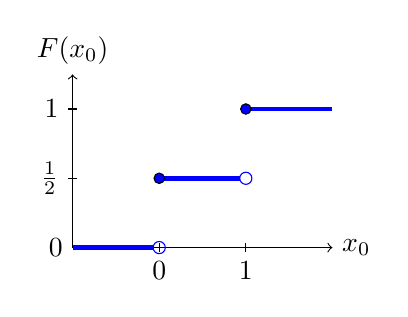
\begin{tikzpicture}[scale = 1.1]
\draw [<->] (0,2) node [above]{$F(x_0)$} -- (0,0) -- (3,0) node [right]{$x_0$};
\draw (-0.05, 1.6) node [black, left]{$1$} -- (0.05,1.6);
\draw (-0.05, 0.8) node [black, left]{$\frac{1}{2}$} -- (0.05,0.8);
\draw [blue, ultra thick] (0,0) -- (0.93,0);
\draw [blue, ultra thick] (1,0.8) -- (1.93,0.8);
\draw [blue, ultra thick] (2,1.6) -- (3,1.6);
\draw (1,-0.05) node [black, below]{0} -- (1,0.05);
\draw (2,-0.05) node [black, below]{1} -- (2,0.05);
\draw (0,0) node [black, left]{$0$};
\draw [blue] (1,0) circle [radius = 0.07];
\draw [fill = blue] (1,0.8) circle [radius = 0.06];
\draw [blue] (2,0.8) circle [radius = 0.07];
\draw [fill = blue] (2,1.6) circle [radius = 0.06];
\end{tikzpicture}
\begin{eqnarray*}
	F(x_0) = \left\{\begin{array}{ll} 0,& x_0 < 0\\ \frac{1}{2}, &0\leq x_0 < 1\\ 1,& x_0 \geq 1\end{array}\right.
\end{eqnarray*}
	\end{block}
\end{columns}
\end{frame}

%%%%%%%%%%%%%%%%%%%%%%%%%%%%%%%%%%%%%%%%

\begin{frame}
\frametitle{Properties of CDFs}
\framesubtitle{These are also true for continuous RVs.}
	\begin{enumerate}
		\item $\lim_{x_0 \rightarrow \infty} F(x_0) = 1$
		\item $\lim_{x_0 \rightarrow -\infty} F(x_0) = 0$
		\item Non-decreasing: $x_0 < x_1 \Rightarrow F(x_0)\leq F(x_1)$
		\item Right-continuous (``open'' versus ``closed'' on prev.\ slide)
	\end{enumerate}
	
\vspace{1em}
\begin{alertblock}{Since $F(x_0) = P(X\leq x_0)$,  we have $0\leq F(x_0)\leq 1$ for all $x_0$}\end{alertblock}
\end{frame}

\section{Lotteries}
%%%%%%%%%%%%%%%%%%%%%%%%%%%%%%%%%%%%%%%%
\begin{frame}
\frametitle{Easy Lottery}
Choose between the following two lotteries:
\begin{itemize}
	\item \textbf{Lottery A:} 
	\begin{itemize}
		\item You get \$1 million for sure
	\end{itemize}
	\item \textbf{Lottery B:}
	\begin{itemize}
		\item 10\% chance of \$5 million
		\item 89\% chance of \$1 million
		\item 1\% chance of nothing
	\end{itemize}	 
\end{itemize}
\end{frame}

%%%%%%%%%%%%%%%%%%%%%%%%%%%%%%%%%%%%%%%%
\begin{frame}
\frametitle{Hard Lottery}
Choose between the following two lotteries:
\begin{itemize}
	\item \textbf{Lottery C:} 
	\begin{itemize}
		\item 11\% chance of \$1 million
		\item 89\% chance of nothing
	\end{itemize}
	\item \textbf{Lottery D:}
	\begin{itemize}
		\item 10\% chance of \$5 million
		\item 90\% chance of nothing
	\end{itemize}	 
\end{itemize}
\end{frame}

%%%%%%%%%%%%%%%%%%%%%%%%%%%%%%%%%%%%%%%%
\begin{frame}
\frametitle{Highly Illogical}
\begin{center}
	
\includegraphics[width = 0.7\textwidth]{./images/spock.jpg}
\end{center}

If you chose $\{A, D\}$ or $\{B, C\}$, you are highly illogical.
\end{frame}

\section{Expectation}
%%%%%%%%%%%%%%%%%%%%%%%%%%%%%%%%%%%%%%%%
\begin{frame}
\frametitle{Expected Value (aka Expectation)}
The expected value of a discrete RV $X$ is given by
	$$E[X] = \sum_{\mbox{all} \; x} x \cdot p(x)$$

  \alert{In other words, the expected value of a discrete RV is the \emph{probability-weighted average of its realizations}.}

  \begin{block}{Notation}
    We sometimes write $\mu$ as shorthand for $E[X]$.  \end{block}
\end{frame}

%%%%%%%%%%%%%%%%%%%%%%%%%%%%%%%%%%%%%%%%
\begin{frame}
\frametitle{How Can I Think About Expected Value?}

\begin{itemize}
	\item The long-run average of a random variable
	\item How much you expect to win from a gamble where the payoffs are the values of the RV
\end{itemize}

If the realizations of the coin-flip RV were \alert{payoffs}, how much would you expect to win per play \emph{on average} in a long sequence of plays?
$$X = \left\{ \begin{array}{l}  \$0, \mbox{Tails}\\ \$1, \mbox{Heads}\end{array} \right.$$
\end{frame}

%%%%%%%%%%%%%%%%%%%%%%%%%%%%%%%%%%%%%%%%
\begin{frame}
  \frametitle{Your Turn to Calculate an Expected Value}
  Let $X$ be a random variable with support set $\left\{ 1,2,3 \right\}$ where $p(1)=p(2)=1/3$. Calculate $E[X]$.

  \pause

  \vspace{1em}
  \begin{equation*}
    E[X] = \sum_{\mbox{all }x} x \cdot p(x) = 1 \times 1/3 + 2 \times 1/3 + 3 \times 1/3 = 2
  \end{equation*}
\end{frame}

%%%%%%%%%%%%%%%%%%%%%%%%%%%%%%%%%%%%%%%%

\begin{frame}
\frametitle{Expectation of a Function of a Discrete RV}
Let $X$ be a random variable and $g$ be a function. Then:
$$\boxed{E[g(X)] = \sum_{\mbox{all } x} g(x) p(x)}$$

Is $E[g(X)] = g(E[X])$? What if $g(x) = x^2$?
\end{frame}

%%%%%%%%%%%%%%%%%%%%%%%%%%%%%%%%%%%%%%%%
\begin{frame}
\frametitle{\alert{IMPORTANT}}
\huge $$E[g(X)] \neq g(E[X])$$
\begin{center}
	\large (Expected Value of Function $\neq$ Function of Expected Value)
\end{center}
\end{frame}

%%%%%%%%%%%%%%%%%%%%%%%%%%%%%%%%%%%%%%%%
\begin{frame}
\frametitle{Linearity of Expectation}
\begin{center}
\fbox{$E[a + bX] = a + bE[X]$}
\end{center}
\only<2->{\textbf{Proof:} 
\begin{align*}
	E[a + bX] &= \sum_{\mbox{all } x}  (a + bx) p(x)\\
	 &=  \sum_{\mbox{all } x} p(x) \cdot a + \sum_{\mbox{all } x}p(x) \cdot bx\\
	&=  a\sum_{\mbox{all } x} p(x) + b\sum_{\mbox{all } x} x \cdot p(x) \\
	&=  a + b E[X]
\end{align*}
One of the few instances where $E[g(X)] = g(E[X])$}

\end{frame}

%%%%%%%%%%%%%%%%%%%%%%%%%%%%%%%%%%%%%%%%
\begin{frame}
\frametitle{Why Was I Highly Illogical?}
This is known as the Allais paradox. 

Let $U(x)$ be the utility you get from money (notice, we are not assuming that every dollar is worth the same to you). 

If you chose A, then we know that
$$
U(1) > 0.1 U(5) + 0.89 U(1) + 0.01 U(0)
$$

\only<2->{If you also chose D, then we know that
\begin{align*}
	0.1 U(5) + 0.9 U(0) &> 0.11 U(1) + 0.89 U(0)
	\\
	0.1 U(5) + 0.89 U(1) + 0.01 U(0) &> U(1)
\end{align*}}

\end{frame}

%%%%%%%%%%%%%%%%%%%%%%%%%%%%%%%%%%%%%%%%
\begin{frame}
\frametitle{Which Is It?}
\centering

\includegraphics[width = 0.84\textwidth]{./images/howToFeel.jpg}
\end{frame}

\section{Variance}
%%%%%%%%%%%%%%%%%%%%%%%%%%%%%%%%%%%%%%%%
\begin{frame}
\frametitle{Variance and Standard Deviation of a RV}

\begin{block}{Variance (Var)}
	$$\sigma^2 = Var(X) = E\left[ (X - \mu)^2\right] = E\left[ (X - E[X])^2\right]$$
\end{block}


\begin{block}{Standard Deviation (SD)}
$$\sigma = \sqrt{\sigma^2} = SD(X)$$
\end{block}

\alert{These look similar to their definitions from last chapter}

\only<2->{\alert{Variance and std.\ dev.\ are \emph{expectations of functions of a RV}}}

\end{frame}

%%%%%%%%%%%%%%%%%%%%%%%%%%%%%%%%%%%%%%%%
\begin{frame}
\frametitle{How To Calculate Variance for Discrete RV?}
\begin{align*}
Var(X) &= E\left[ (X - \mu)^2 \right] =\sum_{\mbox{all } x} (x - \mu)^2 p(x)
\\
&= \sum_{\text{all }x} (x^2 - 2x\mu + \mu^2)p(x) 
\\
&= \sum_{\text{all }x}x^2 p(x) - 2\mu \sum_{\text{all }x}x p(x) + \mu^2 \sum_{\text{all }x} p(x)
\\
&= E[X^2] - 2\mu E[X] + \mu^2
\\
&= E[X^2] - (E[X])^2
\end{align*}

\end{frame}
%%%%%%%%%%%%%%%%%%%%%%%%%%%%%%%%%%%%%%%%
\begin{frame}
\frametitle{Shortcut Formula For Variance}

This is \emph{not} the definition, it's a shortcut for doing calculations:
\begin{eqnarray*}
	Var(X) = E\left[ (X - \mu)^2 \right] = E[X^2] - \left(E[X]\right)^2
\end{eqnarray*}
\end{frame}

%%%%%%%%%%%%%%%%%%%%%%%%%%%%%%%%%%%%%%%%
\begin{frame}
\frametitle{Variance of a Linear Function}
Suppose $X$ is a random variable with $Var(X) = \sigma^2$ and $a,b$ are constants. What is $Var(a + bX)$? 
\begin{enumerate}[(a)]
	\item $\sigma^2$
	\item $a + \sigma^2$
	\item $b \sigma^2$
	\item $a + b \sigma^2$
	\item $b^2 \sigma^2$
\end{enumerate}

\end{frame}
%%%%%%%%%%%%%%%%%%%%%%%%%%%%%%%%%%%%%%%%
\begin{frame}
	\frametitle{Variance and SD are \emph{NOT} Linear}

\begin{eqnarray*}
Var(a + bX) &= &b^2 \sigma^2 \\\\
	SD(a + bX)&=& |b| \sigma
\end{eqnarray*}

\vspace{2em}
\begin{block}{These should look familiar from the related results for sample variance and std.\ dev. that you worked out on an earlier problem set.}

\end{block}

\end{frame}
%%%%%%%%%%%%%%%%%%%%%%%%%%%%%%%%%%%%%%%%
\begin{frame}
\frametitle{Variance of a Linear Transformation}

\begin{eqnarray*}
 Var(a + bX) &=& E\left[\left\{(a+bX) - E(a+bX)\right\}^2 \right] \\ 
 	&=& E\left[\left\{(a+bX) - (a+bE[X])\right\}^2 \right] \\
 	&=&E\left[\left(bX - bE[X]\right)^2 \right] \\ 
 	&=&E[b^2 (X - E[X])^2]\\ 
 	&=& b^2 E[(X-E[X])^2]\\ 
 	&=& b^2 Var(X) = b^2 \sigma^2
\end{eqnarray*}
\alert{The key point here is that variance is defined in terms of expectation and expectation is linear.}

\end{frame}

%%%%%%%%%%%%%%%%%%%%%%%%%%%%%%%%%%%%%%%%
\begin{frame}
\frametitle{Constants Versus Random Variables}

 \alert{This is a crucial distinction that students sometimes miss:}

 		\begin{itemize}
 			\item \textbf{Random Variables}
 			\begin{itemize}
	 			\item Suppose $X$ is a RV -- the values it takes on are random
 				\item A function $g(X)$ of a RV is itself a RV
 			\end{itemize} 
 			\item \textbf{Constants}
 			\begin{itemize}
 				\item $E[X]$ and $Var(X)$ are constants
 				\item Realizations $x$ are constants, but \emph{which} realization the RV takes on is random
 				\item Parameters are constants
 				\item Sample size $n$ is a constant
 			\end{itemize}
 		\end{itemize} 
\end{frame}

\section{Bernoulli Random Variable}
%%%%%%%%%%%%%%%%%%%%%%%%%%%%%%%%%%%%%%%%
\begin{frame}
\frametitle{Bernoulli Random Variable -- Generalization of Coin Flip}
\small
\begin{block}{Support Set}
$\{0,1\}$ -- 1 traditionally called ``success,'' 0 ``failure''
\end{block}

\begin{block}{Probability Mass Function}
	\begin{eqnarray*}
		p(0) &=& 1-p\\
		p(1) &=& p
	\end{eqnarray*}

	\begin{block}{Cumulative Distribution Function}
\begin{eqnarray*}
	F(x_0) = \left\{\begin{array}{ll} 0,& x_0 < 0\\ 1-p, &0\leq x_0 < 1\\ 1,& x_0 \geq 1\end{array}\right.
\end{eqnarray*}
\end{block}
\end{block}

\end{frame}

%%%%%%%%%%%%%%%%%%%%%%%%%%%%%%%%%%%%%%%%
\begin{frame}
  \frametitle{Expected Value of Bernoulli RV}
$$X = \left\{ \begin{array}{l}  0, \mbox{Failure: } 1-p\\ 1, \mbox{Success: } p\end{array} \right.$$

\vspace{2em}
 
$$\sum_{\mbox{all} \; x} x \cdot p(x) = 0 \cdot (1-p) + 1 \cdot p = p$$
\end{frame}

%%%%%%%%%%%%%%%%%%%%%%%%%%%%%%%%%%%%%%%%
\begin{frame}
\frametitle{Variance of Bernoulli RV -- via the Shortcut Formula}

\begin{block}{Step 1 -- $E[X]$} 
$\mu = E[X] = \displaystyle \sum_{x \in \{0,1\}} p(x) \cdot x = (1-p) \cdot 0 + p \cdot 1 = p$
\end{block}


\begin{block}{Step 2 -- $E[X^2]$} 
\begin{eqnarray*}
	E[X^2] = \sum_{x \in \{0,1\}} x^2 p(x) = 0^2 (1-p) + 1^2 p = p
\end{eqnarray*}
\end{block}


\begin{block}{Step 3 -- Combine with Shortcut Formula} 
\begin{eqnarray*}
	\sigma^2 = Var[X] = E[X^2] - \left(E[X]\right)^2 = \ p - p^2 =  p(1-p)
\end{eqnarray*}
\end{block}


\end{frame}

%%%%%%%%%%%%%%%%%%%%%%%%%%%%%%%%%%%%%%%%
\begin{frame}
\frametitle{Variance of Bernoulli RV -- Without Shortcut}

\alert{You will fill in the missing steps on Problem Set 5.}

\begin{eqnarray*}
	\sigma^2 &=& Var(X) = \sum_{x \in \{0,1\}} (x - \mu)^2 p(x)\\
	 &=& \sum_{x \in \{0,1\}} (x - p)^2 p(x)\\
	 &\vdots &\\ 
	 &=&p(1-p)
\end{eqnarray*}
\end{frame}

%%%%%%%%%%%%%%%%%%%%%%%%%%%%%%%%%%%%%%%%

\begin{frame}
\frametitle{Random Variables and Parameters}



\begin{block}{Notation: $X \sim$ Bernoulli$(p)$}
Means $X$ is a Bernoulli RV with $P(X = 1) = p$ and $P(X= 0) = 1-p$. The tilde is read ``distributes as.''

\end{block}


\begin{block}{Parameter}
Any constant that appears in the definition of a RV, here $p$. 
\end{block}


\end{frame}

\section{The St.\ Petersburg Game}
%%%%%%%%%%%%%%%%%%%%%%%%%%%%%%%%%%%%%%%%
\begin{frame}
\frametitle{How Much Would You Pay?}
How much would you be willing to pay for the right to play the following game?

\vspace{1em}
\begin{quote}
Imagine a fair coin. The coin is tossed once. If it falls heads, you receive a prize of \$2 and the game stops. If not, it is tossed again. If it falls heads on the second toss, you get \$4 and the game stops. If not, it is tossed again. If it falls heads on the third toss, you get \$8 and the game stops, and so on. The game stops after the first head is thrown. If the first head is thrown on the $x^{th}$ toss, the prize is \$$2^x$
\end{quote}

\end{frame}

%%%%%%%%%%%%%%%%%%%%%%%%%%%%%%%%%%%%%%%%
\begin{frame}
\frametitle{$X =$ Trial Number of First Head}
\begin{table}
\begin{tabular}{c|c|c|c}
	$x$ & $2^x$ & $p(x)$& $2^x \cdot p(x)$\\
		\hline \uncover<2->{
	1&2&1/2&1\\
	2&4&1/4&1\\
	3&8&1/8&1\\}\uncover<3->{
	$\vdots$&$\vdots$&$\vdots$&$\vdots$\\
	n&$2^n$&$1/2^n$&1\\
	$\vdots$&$\vdots$&$\vdots$&$\vdots$}
\end{tabular}
\end{table}
$$E[Y] = \sum_{\mbox{all } x} 2^x\cdot p(x) = \uncover<4->{1 + 1 + 1 + \hdots}\uncover<5->{ = \infty}$$
\end{frame}

\section{Functions of Random Variables}
%%%%%%%%%%%%%%%%%%%%%%%%%%%%%%%%%%%%%%%%

\begin{frame}
\frametitle{Example: Function of Bernoulli RV}
\fbox{Let $Y=e^X$ where $X \sim \mbox{Bernoulli}(p)$}
\vspace{2em}

\begin{block}{Support of $Y$} \pause
$\{e^0, e^1\} =\{1, e\}$
\end{block}

\begin{block}{Probability Mass Function for $Y$} \pause
	$$p_Y(y) = \left\{\begin{array}{ll}p& y =e\\ 1-p& y = 1\\ 0& \mbox{otherwise}\end{array}\right.$$
\end{block}

\end{frame}
%%%%%%%%%%%%%%%%%%%%%%%%%%%%%%%%%%%%%%%%
\begin{frame}
\frametitle{Expectation: Function of Bernoulli RV}
\fbox{Let $Y=e^X$ where $X \sim \mbox{Bernoulli}(p)$}
\vspace{2em}

\begin{block}{Probability Mass Function for $Y$} 
	$$p_Y(y) = \left\{\begin{array}{ll}p& y =e\\ 1-p& y = 1\\ 0& \mbox{otherwise}\end{array}\right.$$
\end{block}

\begin{block}{Expectation of $Y = e^X$}\pause
$$\sum_{y \in \{1, e\}} y \cdot p_Y(y) =\pause (1-p) \cdot 1 + p \cdot e = 1 + p(e - 1)$$
\end{block}




\end{frame}
%%%%%%%%%%%%%%%%%%%%%%%%%%%%%%%%%%%%%%%%
\begin{frame}
\frametitle{Expectation: Function of Bernoulli RV}
\fbox{Let $Y=e^X$ where $X \sim \mbox{Bernoulli}(p)$}
\vspace{2em}



\begin{block}{Expectation of the Function}
$$\sum_{y \in \{1, e\}} y \cdot p_Y(y) = (1-p) \cdot 1 + p \cdot e = 1 + p(e - 1)$$
\end{block}

\begin{block}{Function of the Expectation}
$$e^{E[X]} = e^p $$
\end{block}



\end{frame}

\section{Binomial Random Variable}
%%%%%%%%%%%%%%%%%%%%%%%%%%%%%%%%%%%%%%%%
\begin{frame}
\frametitle{Binomial Random Variable}
Let $X = $ the sum of $n$ independent Bernoulli trials, each with probability of success $p$.  \alert{Then we say that:
		$X \sim \mbox{Binomial}(n,p)$} 

\vspace{2em}
\begin{block}{Parameters}
$p =$ probability of ``success,'' $n=$ \# of trials
\end{block}
\begin{block}{Support} 
$\{0, 1, 2, \hdots, n\}$ 
\end{block}
\begin{block}{Probability Mass Function (PMF)} 
$$p(x) = \binom{n}{x} p^x (1-p)^{n-x}$$ 
\end{block}
\end{frame}

%%%%%%%%%%%%%%%%%%%%%%%%%%%%%%%%%%%%%%%%
\begin{frame}
\frametitle{Where does the Binomial PMF come from? }
\begin{block}{Question}
Let's flip a fair coin 3 times. What is the probability that we get exactly 2 heads?
\end{block}

\pause

\begin{block}{Answer}
Three basic outcomes make up this event: $\{HHT, HTH, THH\}$, each has probability $1/8 = 1/2 \times 1/2 \times 1/2$. Basic outcomes are mutually exclusive, so sum to get \alert{$3/8 = 0.375$}
\end{block}

\end{frame}
%%%%%%%%%%%%%%%%%%%%%%%%%%%%%%%%%%%%%%%%
\begin{frame}
\frametitle{Where does the Binomial PMF come from?}
\begin{block}{Question}
Let's flip an \emph{unfair} coin 3 times, where the probability of heads is 1/3. What is the probability that we get exactly 2 heads?
\end{block}



\begin{block}{Answer}
  \emph{All} basic outcomes are not equally likely, but those with exactly two heads \emph{\alert{still are}} 
	\begin{eqnarray*}
	 P(HHT) &=&  (1/3)^2 (1 - 1/3) =  2/27\\ 
	 P(THH) &=&2/27\\ 
	 P(HTH) &=&2/27 
	\end{eqnarray*}
	Summing gives \alert{$2/9 \approx 0.22$}
\end{block}
\end{frame}

%%%%%%%%%%%%%%%%%%%%%%%%%%%%%%%%%%%%%%%%
\begin{frame}
  \frametitle{Where does the Binomial PMF come from?}

Suppose we flip an unfair coin \emph{4} times, where the probability of heads is 1/3. What is the probability that we get exactly 2 heads?

\vspace{2em}



\begin{columns}
\column{0.35\textwidth}
\begin{tabular}{cc}
HHTT&TTHH\\
HTHT&THTH\\
HTTH&THHT
\end{tabular}

\column{0.55\textwidth}
\alert{Six equally likely, mutually exclusive basic outcomes make up this event:}
$$\binom{4}{2}(1/3)^2(2/3)^2$$
\end{columns}

\end{frame}

\section{Joint Distributions}
%%%%%%%%%%%%%%%%%%%%%%%%%%%%%%%%%%%%%%%%
\begin{frame}
  \frametitle{Definition}
  Sometimes we are interested in how two random variables behave together (aka jointly). Because of this, we need a way to characterize their joint behavior.
  
	\textbf{Joint probability mass function ($p_{XY}(x, y)$):} Let $X$ and $Y$ be discrete random variables. The joint probability mass function $p_{XY}(x,y)$ gives the probability of each pair of realizations $(x,y)$ in the support:

\Large
 $$\boxed{p_{XY}(x,y) = P(X = x \cap Y=y)}$$

\end{frame}
%%%%%%%%%%%%%%%%%%%%%%%%%%%%%%%%%%%%%%%%
\begin{frame}
\frametitle{Example: Joint PMF in Tabular Form}

\alert{For discrete RVs, we often use tables}

\begin{table}
\begin{tabular}{|cc|ccc|}
\hline
&&\multicolumn{3}{c|}{$Y$}\\
&&1 & 2&3\\
\hline
\multirow{4}{*}{$X$}
&0& \multicolumn{1}{c}{\alert{1/8}} & \alert{0}& \alert{0}\\
&1& \multicolumn{1}{c}{\alert{0}} & \alert{1/4}&\alert{1/8}\\
&2& \multicolumn{1}{c}{\alert{0}} & \alert{1/4}&\alert{1/8}\\
&3& \multicolumn{1}{c}{\alert{1/8}} & \alert{0}&\alert{0}\\
\hline
\end{tabular}
\end{table}

One example might be that $X$ is one's home region (0 is Northeast, 1 is Northwest, 2 is Southeast, 3 is Southwest) and $Y$ is the car they own (1 is sedan, 2 is SUV, 3 is truck).

\end{frame}

%%%%%%%%%%%%%%%%%%%%%%%%%%%%%%%%%%%%%%%%
\begin{frame}
\frametitle{Plot of Joint PMF}
\begin{figure}
	\includegraphics[scale = 0.44]{./images/joint_dist}
\end{figure}

\end{frame}



%%%%%%%%%%%%%%%%%%%%%%%%%%%%%%%%%%%%%%%%
\begin{frame}
\frametitle{What is $p_{XY}(1,2)$?}

\begin{table}
\begin{tabular}{|cc|ccc|}
\hline
&&\multicolumn{3}{c|}{$Y$}\\
&&1 & 2&3\\
\hline
\multirow{4}{*}{$X$}
&0& \multicolumn{1}{c}{\alert{1/8}} & \alert{0}& \alert{0}\\
&1& \multicolumn{1}{c}{\alert{0}} & \alert{1/4}&\alert{1/8}\\
&2& \multicolumn{1}{c}{\alert{0}} & \alert{1/4}&\alert{1/8}\\
&3& \multicolumn{1}{c}{\alert{1/8}} & \alert{0}&\alert{0}\\
\hline
\end{tabular}
\end{table}

\pause



$$p_{XY}(1,2) =   P(X=1 \cap Y =2) =  \alert{1/4}$$

\end{frame}

%%%%%%%%%%%%%%%%%%%%%%%%%%%%%%%%%%%%%%%%
\begin{frame}
\frametitle{What is $p_{XY}(2,1)$?}

\begin{table}
\begin{tabular}{|cc|ccc|}
\hline
&&\multicolumn{3}{c|}{$Y$}\\
&&1 & 2&3\\
\hline
\multirow{4}{*}{$X$}
&0& \multicolumn{1}{c}{\alert{1/8}} & \alert{0}& \alert{0}\\
&1& \multicolumn{1}{c}{\alert{0}} & \alert{1/4}&\alert{1/8}\\
&2& \multicolumn{1}{c}{\alert{0}} & \alert{1/4}&\alert{1/8}\\
&3& \multicolumn{1}{c}{\alert{1/8}} & \alert{0}&\alert{0}\\
\hline
\end{tabular}
\end{table}

\pause

$$p_{XY}(2,1) =  P(X=2 \cap Y =1) = \alert{0}$$

\end{frame}

%%%%%%%%%%%%%%%%%%%%%%%%%%%%%%%%%%%%%%%%

\begin{frame}
\frametitle{Properties of Joint PMF}
	\begin{enumerate}
		\item $0\leq p_{XY}(x,y)\leq 1$ for any pair $(x,y)$
		\item The sum of $p_{XY}(x,y)$ over all pairs $(x,y)$ in the support is 1:
			$$\sum_{x}\sum_{y} p(x,y) = 1$$
	\end{enumerate}
\end{frame}


%%%%%%%%%%%%%%%%%%%%%%%%%%%%%%%%%%%%%%%%
\begin{frame}
\frametitle{Does this satisfy the properties of a joint PMF?}
\begin{table}
\begin{tabular}{|cc|ccc|}
\hline
&&\multicolumn{3}{c|}{$Y$}\\
&&1 & 2&3\\
\hline
\multirow{4}{*}{$X$}
&0& \multicolumn{1}{c}{\alert{1/8}} & \alert{0}& \alert{0}\\
&1& \multicolumn{1}{c}{\alert{0}} & \alert{1/4}&\alert{1/8}\\
&2& \multicolumn{1}{c}{\alert{0}} & \alert{1/4}&\alert{1/8}\\
&3& \multicolumn{1}{c}{\alert{1/8}} & \alert{0}&\alert{0}\\
\hline
\end{tabular}
\end{table}

\pause

\begin{enumerate}
	\item $p(x,y) \geq 0$ for all pairs $(x,y)$
	\item $\sum_x\sum_{y} p(x,y) = 1/8 + 1/4 + 1/8 + 1/4 + 1/8 + 1/8 = 1$
\end{enumerate}

\end{frame}

%%%%%%%%%%%%%%%%%%%%%%%%%%%%%%%%%%%%%%%%
\begin{frame}
\frametitle{Joint versus Marginal PMFs}

What if we just care about one RV? Then, use the \alert{marginal PMF}

\begin{block}{Marginal PMFs}
$p_X(x) = P(X=x)$\\ $p_Y(y) = P(Y=y)$
\end{block}



\vspace{1em}

\alert{You can't calculate a joint pmf from marginals alone but you \emph{can} calculate marginals from the joint!}

\end{frame}
%%%%%%%%%%%%%%%%%%%%%%%%%%%%%%%%%%%%%%%%
\begin{frame}
\frametitle{Marginals from Joint}
	$$
	\boxed{p_X(x) = \sum_{\mbox{all } y} p_{XY}(x,y)}  \quad	\boxed{p_Y(y) = \sum_{\mbox{all } x} p_{XY}(x,y)}
	$$
	
	\begin{block}{Why?}
	\begin{eqnarray*}
	p_Y(y) &=& P(Y=y) = P\left( \bigcup_{\mbox{all } x}\left\{ X=x \cap Y=y \right\}  \right)\\
		&=& \sum_{\mbox{all } x} P(X=x \cap Y=y) = \sum_{\mbox{all } x} p_{XY}(x,y)
	\end{eqnarray*}
	\end{block}
\end{frame}
%%%%%%%%%%%%%%%%%%%%%%%%%%%%%%%%%%%%%%%%
\begin{frame}
\frametitle{To get the marginals sum ``into the margins'' of the table.}

\begin{center}
\begin{tabular}{|cc|ccc|c|}
\hline
&&\multicolumn{3}{c|}{$Y$}&\\
&&1 & 2&3&\\
\hline
\multirow{4}{*}{$X$}
&0& \multicolumn{1}{c}{\alert{1/8}} & \alert{0}& \alert{0}&\onslide<2->{\textcolor{blue}{1/8}}\\
&1& \multicolumn{1}{c}{\alert{0}} & \alert{1/4}&\alert{1/8}&\onslide<3->{\textcolor{blue}{3/8}}\\
&2& \multicolumn{1}{c}{\alert{0}} & \alert{1/4}&\alert{1/8}&\onslide<4->{\textcolor{blue}{3/8}}\\
&3& \multicolumn{1}{c}{\alert{1/8}} & \alert{0}&\alert{0}&\onslide<5->{\textcolor{blue}{1/8}}\\
\hline 
&&&&&\onslide<5->{\textcolor{blue}{1}}\\
\hline
\end{tabular}
\end{center}

\begin{eqnarray*}
	\onslide<2->{p_X(0) &=& 1/8 + 0 + 0 = 1/8}\\
	\onslide<3->{p_X(1) &=&0 + 1/4 + 1/8 = 3/8}\\
	\onslide<4->{p_X(2) &=&0 + 1/4 + 1/8 = 3/8}\\
	\onslide<5->{p_X(3) &=&1/8 + 0 + 0 = 1/8}
\end{eqnarray*}


\end{frame}

%%%%%%%%%%%%%%%%%%%%%%%%%%%%%%%%%%%%%%%%

\begin{frame}
\frametitle{Marginal Probabilities}

\begin{table}
\begin{tabular}{|cc|ccc|c|}
\hline
&&\multicolumn{3}{c|}{$Y$}&\\
&&1 & 2&3&\\
\hline
\multirow{4}{*}{$X$}
&0& \multicolumn{1}{c}{\alert{1/8}} & \alert{0}& \alert{0}&\\
&1& \multicolumn{1}{c}{\alert{0}} & \alert{1/4}&\alert{1/8}&\\
&2& \multicolumn{1}{c}{\alert{0}} & \alert{1/4}&\alert{1/8}&\\
&3& \multicolumn{1}{c}{\alert{1/8}} & \alert{0}&\alert{0}&\\
\hline 
&&\onslide<2->{\textcolor{blue}{1/4}}&\onslide<3->{ \textcolor{blue}{1/2} }& \onslide<4->{\textcolor{blue}{1/4}} &\onslide<4->{\textcolor{blue}{1}}\\
\hline
\end{tabular}
\end{table}

\begin{eqnarray*}
	\onslide<2->{p_Y(1) &=& 1/8 + 0 + 0 + 1/8 = 1/4}\\
	\onslide<3->{p_Y(2) &=&0 + 1/4 + 1/4 + 0 = 1/2}\\
	\onslide<4->{p_Y(3) &=&0 + 1/8 + 1/8 + 0= 1/4}
\end{eqnarray*}


\end{frame}

\section{Conditional Distributions}
%%%%%%%%%%%%%%%%%%%%%%%%%%%%%%%%%%%%%%%%
\begin{frame}
\frametitle{Definition of Conditional PMF}

How does the distribution of $y$ change with $x$? In other words, if we know $x$, does that tell us anything about $y$?

\begin{eqnarray*}
	p_{Y|X}(y|x) = P(Y=y|X=x) =  \frac{P(Y=y \cap X=x)}{P(X=x)} =  \frac{p_{XY}(x,y)}{p_X(x)}
\end{eqnarray*}
\end{frame}


%%%%%%%%%%%%%%%%%%%%%%%%%%%%%%%%%%%%%%%%
\begin{frame}
\frametitle{Conditional PMF of $Y$ given $X = 2$}

\begin{table}
\begin{tabular}{|cc|ccc|c|}
\hline
&&\multicolumn{3}{c|}{$Y$}&\\
&&1 & 2&3&\\
\hline
\multirow{4}{*}{$X$}
&0& \multicolumn{1}{c}{1/8} & 0& 0&1/8\\
&1& \multicolumn{1}{c}{0} & 1/4&1/8&3/8\\
&2& \multicolumn{1}{c}{\alert{0}} & \alert{1/4}&\alert{1/8}&\textcolor{blue}{3/8}\\
&3& \multicolumn{1}{c}{1/8} & 0&0&1/8\\
\hline
\end{tabular}
\end{table}

\begin{eqnarray*}
	p_{Y|X}(1|2) &=& \frac{p_{XY}(2,1)}{p_X(2)} = \frac{0}{3/8} =\alert{0}\\ \\
	p_{Y|X}(2|2) &=&\frac{p_{XY}(2,2)}{p_X(2)}= \frac{1/4}{3/8} =\alert{2/3} \\ \\ 
	 p_{Y|X}(3|2) &=&\frac{p_{XY}(2,3)}{p_X(2)} = \frac{1/8}{3/8} = \alert{1/3}
\end{eqnarray*}


\end{frame}
%%%%%%%%%%%%%%%%%%%%%%%%%%%%%%%%%%%%%%%%
\begin{frame}
\frametitle{What is $p_{X|Y}(1|2)$? }
\small
\begin{table}
\begin{tabular}{|cc|ccc|c|}
\hline
&&\multicolumn{3}{c|}{$Y$}&\\
&&1 & 2&3&\\
\hline
\multirow{4}{*}{$X$}
&0& \multicolumn{1}{c}{1/8} & \alert{0}&0&\\
&1& \multicolumn{1}{c}{0} & \alert{1/4}&1/8&\\
&2& \multicolumn{1}{c}{0} & \alert{1/4}&1/8&\\
&3& \multicolumn{1}{c}{1/8} & \alert{0}&0&\\
\hline 
&&1/4&\textcolor{blue}{1/2}&1/4&\\
\hline
\end{tabular}
\end{table}

\pause
\begin{equation}
	p_{X|Y}(1|2) =\frac{p_{XY}(1,2)}{p_Y(2)}=\frac{1/4}{1/2}= \alert{1/2}
\end{equation}

  \pause

Similarly: 
$$p_{X|Y}(0|2)=0, \quad p_{X|Y}(2|2)=1/2, \quad p_{X|Y}(3|2)= 0$$


\end{frame}

%%%%%%%%%%%%%%%%%%%%%%%%%%%%%%%%%%%%%%%%


\begin{frame}
\frametitle{Independent RVs: Joint Equals Product of Marginals}


\begin{block}{Definition}
  Two discrete RVs are \alert{independent} if and only if
  $$p_{XY}(x,y) = p_X(x)p_Y(y)$$ for all pairs $(x,y)$ in the support.
\end{block}


\begin{block}{Equivalent Definition}
  \vspace{-1em}
  $$p_{Y|X}(y|x) = p_Y(y) \mbox{ and } p_{X|Y}(x|y) = p_X(x)$$
  for all pairs $(x,y)$ in the support.
\end{block}

\end{frame}
%%%%%%%%%%%%%%%%%%%%%%%%%%%%%%%%%%%%%%%%
\begin{frame}
\frametitle{Are $X$ and $Y$ Independent? }
\small
\begin{table}
\begin{tabular}{|cc|ccc|c|}
\hline
&&\multicolumn{3}{c|}{$Y$}&\\
&&1 & 2&3&\\
\hline
\multirow{4}{*}{$X$}
&0& \multicolumn{1}{|c}{\alert{1/8}} & \alert{0}& \alert{0}&\textcolor{blue}{1/8}\\
&1& \multicolumn{1}{|c}{\alert{0}} & \alert{1/4}&\alert{1/8}&\textcolor{blue}{3/8}\\
&2& \multicolumn{1}{|c}{\alert{0}} & \alert{1/4}&\alert{1/8}&\textcolor{blue}{3/8}\\
&3& \multicolumn{1}{|c}{\alert{1/8}} & \alert{0}&\alert{0}&\textcolor{blue}{1/8}\\
\hline
&&\textcolor{blue}{1/4}&\textcolor{blue}{1/2}&\textcolor{blue}{1/4}&\\
\hline
\end{tabular}
\end{table}

\pause

\begin{eqnarray*}
	p_{XY}(2,1) &=& 0\\ 
	p_X(2) \times p_Y(1) &=&  (3/8) \times (1/4) \neq 0
\end{eqnarray*}

\alert{Therefore $X$ and $Y$ are \emph{not} independent.}
\end{frame}

\section{Conditional Expectation}
%%%%%%%%%%%%%%%%%%%%%%%%%%%%%%%%%%%%%%%%
\begin{frame}
\frametitle{Conditional Expectation}
\begin{block}{Intuition}
	$E[Y|X] = $ ``best guess'' of realization that $Y$ after observing realization of $X$. 
\end{block}

\begin{block}{$E[Y|X]$ is a Random Variable}
While $E[Y]$ is a constant, $E[Y|X]$ is a function of $X$, hence a \alert{Random Variable}.
\end{block}

\begin{block}{$E[Y|X=x]$ is a Constant}
  The constant $E[Y|X=x]$ is the ``guess'' of $Y$ if we see $X=x$.
\end{block}

\begin{block}{Calculating $E[Y|X=x]$}
Take the mean of the conditional pmf of $Y$ given $X=x$.
\end{block}

\end{frame}
%%%%%%%%%%%%%%%%%%%%%%%%%%%%%%%%%%%%%%%%
\begin{frame}
	\frametitle{Conditional Expectation: $E[Y|X=2]$}

\footnotesize
\begin{table}
\begin{tabular}{|cc|ccc|c|}
\hline
&&\multicolumn{3}{c|}{$Y$}&\\
&&1 & 2&3&\\
\hline
\multirow{4}{*}{$X$}
&0& \multicolumn{1}{c}{\alert{1/8}} & \alert{0}& \alert{0}&\textcolor{blue}{1/8}\\
&1& \multicolumn{1}{c}{\alert{0}} & \alert{1/4}&\alert{1/8}&\textcolor{blue}{3/8}\\
&2& \multicolumn{1}{c}{\alert{0}} & \alert{1/4}&\alert{1/8}&\textcolor{blue}{3/8}\\
&3& \multicolumn{1}{c}{\alert{1/8}} & \alert{0}&\alert{0}&\textcolor{blue}{1/8}\\
\hline
&&\textcolor{blue}{1/4}&\textcolor{blue}{1/2}&\textcolor{blue}{1/4}&\\
\hline
\end{tabular}
\end{table}

We showed above that the conditional pmf of $Y|X=2$ is:
	$$\boxed{\begin{array}{ccc}p_{Y|X}(1|2) =0 \quad&p_{Y|X}(2|2) =2/3 \quad&p_{Y|X}(3|2) =1/3\end{array}}$$
	
	
Hence
	$$E[Y|X=2] = 2 \times 2/3 + 3 \times 1/3 =  \alert{7/3}$$

\end{frame}
%%%%%%%%%%%%%%%%%%%%%%%%%%%%%%%%%%%%%%%%
\begin{frame}
	\frametitle{Conditional Expectation: $E[Y|X=0]$}

\footnotesize
\begin{table}
\begin{tabular}{|cc|ccc|c|}
\hline
&&\multicolumn{3}{c|}{$Y$}&\\
&&1 & 2&3&\\
\hline
\multirow{4}{*}{$X$}
&0& \multicolumn{1}{c}{\alert{1/8}} & \alert{0}& \alert{0}&\textcolor{blue}{1/8}\\
&1& \multicolumn{1}{c}{\alert{0}} & \alert{1/4}&\alert{1/8}&\textcolor{blue}{3/8}\\
&2& \multicolumn{1}{c}{\alert{0}} & \alert{1/4}&\alert{1/8}&\textcolor{blue}{3/8}\\
&3& \multicolumn{1}{c}{\alert{1/8}} & \alert{0}&\alert{0}&\textcolor{blue}{1/8}\\
\hline
&&\textcolor{blue}{1/4}&\textcolor{blue}{1/2}&\textcolor{blue}{1/4}&\\
\hline
\end{tabular}
\end{table}

The conditional pmf of $Y|X=0$ is 
	$$\boxed{\begin{array}{ccc}p_{Y|X}(1|0) =1 \quad&p_{Y|X}(2|0) =0 \quad&p_{Y|X}(3|0) =0\end{array}}$$
	

\alert{Hence $E[Y|X=0] = 1$}

\end{frame}
%%%%%%%%%%%%%%%%%%%%%%%%%%%%%%%%%%%%%%%%
\begin{frame}
	\frametitle{Calculate $E[Y|X=3]$}

\footnotesize
\begin{table}
\begin{tabular}{|cc|ccc|c|}
\hline
&&\multicolumn{3}{c|}{$Y$}&\\
&&1 & 2&3&\\
\hline
\multirow{4}{*}{$X$}
&0& \multicolumn{1}{c}{\alert{1/8}} & \alert{0}& \alert{0}&\textcolor{blue}{1/8}\\
&1& \multicolumn{1}{c}{\alert{0}} & \alert{1/4}&\alert{1/8}&\textcolor{blue}{3/8}\\
&2& \multicolumn{1}{c}{\alert{0}} & \alert{1/4}&\alert{1/8}&\textcolor{blue}{3/8}\\
&3& \multicolumn{1}{c}{\alert{1/8}} & \alert{0}&\alert{0}&\textcolor{blue}{1/8}\\
\hline
&&\textcolor{blue}{1/4}&\textcolor{blue}{1/2}&\textcolor{blue}{1/4}&\\
\hline
\end{tabular}
\end{table}


The conditional pmf of $Y|X=3$ is
	$$\boxed{\begin{array}{ccc}p_{Y|X}(1|3) =1 \quad&p_{Y|X}(2|3) =0 \quad&p_{Y|X}(3|3) =0\end{array}}$$
	
\alert{Hence $E[Y|X=3] = 1$}

\end{frame}
%%%%%%%%%%%%%%%%%%%%%%%%%%%%%%%%%%%%%%%%
\begin{frame}
	\frametitle{Calculate $E[Y|X=1]$ }

\footnotesize
\begin{table}
\begin{tabular}{|cc|ccc|c|}
\hline
&&\multicolumn{3}{c|}{$Y$}&\\
&&1 & 2&3&\\
\hline
\multirow{4}{*}{$X$}
&0& \multicolumn{1}{c}{\alert{1/8}} & \alert{0}& \alert{0}&\textcolor{blue}{1/8}\\
&1& \multicolumn{1}{c}{\alert{0}} & \alert{1/4}&\alert{1/8}&\textcolor{blue}{3/8}\\
&2& \multicolumn{1}{c}{\alert{0}} & \alert{1/4}&\alert{1/8}&\textcolor{blue}{3/8}\\
&3& \multicolumn{1}{c}{\alert{1/8}} & \alert{0}&\alert{0}&\textcolor{blue}{1/8}\\
\hline
&&\textcolor{blue}{1/4}&\textcolor{blue}{1/2}&\textcolor{blue}{1/4}&\\
\hline
\end{tabular}
\end{table}
\pause
The conditional pmf of $Y|X=1$ is
	$$\boxed{\begin{array}{ccc}p_{Y|X}(1|1) =0 \quad&p_{Y|X}(2|1) =2/3 \quad&p_{Y|X}(3|1) =1/3\end{array}}$$
	

Hence
	$$E[Y|X=1] = 2 \times 2/3 + 3 \times 1/3 = \alert{7/3}$$

\end{frame}
%%%%%%%%%%%%%%%%%%%%%%%%%%%%%%%%%%%%%%%%
\begin{frame}
\frametitle{$E[Y|X]$ is a Random Variable}
For this example:
	$$E[Y|X]= \left\{\begin{array}{cc}  
	1& X = 0\\
	7/3& X = 1\\
	7/3& X = 2\\ 
	1& X = 3 
	\end{array}\right.$$ 
From above the marginal distribution of $X$ is:
	\begin{eqnarray*}
		P(X=0)= 1/8 && P(X=1) = 3/8\\
		P(X=2)=3/8 && P(X=3)=1/8
	\end{eqnarray*} 
\alert{$E[Y|X]$ takes the value 1 with prob.\ 1/4 and 7/3 with prob.\ 3/4.}

\end{frame}

\section{Law of Iterated Expectations}
%%%%%%%%%%%%%%%%%%%%%%%%%%%%%%%%%%%%%%%%
\begin{frame}
\frametitle{The Law of Iterated Expectations}
Remember that $E[Y|X]$ is a random variable, so it makes sense to ask what its expectation is. It turns out that there's a nice solution:

\Huge
	$$\boxed{E\left[E\left[Y|X  \right]  \right] = E[Y]}$$
\end{frame}

%%%%%%%%%%%%%%%%%%%%%%%%%%%%%%%%%%%%%%%%
\begin{frame}
\frametitle{Proof of The Law of Iterated Expectations (Helpful for 104)}

\begin{eqnarray*}
	E_X\left[ E_{Y|X}\left[Y|X\right] \right] &=&E_X\left[ \sum_y y \; p_{Y|X}(y|x)\right] = \sum_x \left( \sum_y y \; p_{Y|X}(y|x)\right) p_X(x) \\
		&=& \sum_x \sum_y y \; p_X(x) \; p_{Y|X}(y|x) = \sum_x \sum_y y \; p_{XY}(x,y)\\
		&=& \sum_y y \sum_x p_{XY}(x,y) = \sum_y y \;p_Y(y) = E[Y]
\end{eqnarray*}
\end{frame}

%%%%%%%%%%%%%%%%%%%%%%%%%%%%%%%%%%%%%%%%
\begin{frame}[t]
\frametitle{Law of Iterated Expectations for Our Example}

\begin{columns}
\footnotesize
\column{0.5\textwidth}
\begin{block}{Marginal pmf of $Y$}
\begin{eqnarray*}
	P(Y = 1) &=& 1/4 \\
	P(Y = 2) &=& 1/2\\
	P(Y = 3) &=& 1/4
\end{eqnarray*}


\begin{eqnarray*}
	E[Y] &=& 1\times 1/4 + 2 \times 1/2 + 3 \times 1/4\\
		&=&2
\end{eqnarray*}
\end{block}

\column{0.5\textwidth}
\begin{block}{$E[Y|X]$}
	\begin{eqnarray*}
	 E[Y|X] &=& \left\{\begin{array}{cc} 1& \mbox{w/ prob. } 1/4\\ 7/3& \mbox{w/ prob. } 3/4\end{array}\right.\\\\ 
	 E\left[E\left[Y|X \right] \right] &=& 1 \times 1/4 + 7/3 \times 3/4\\ 
	 &=& 2
	\end{eqnarray*}
	\vspace{1em}
\end{block}

\end{columns}

\end{frame}
%%%%%%%%%%%%%%%%%%%%%%%%%%%%%%%%%%%%%%%%
\begin{frame}
\frametitle{Expectation of Function of Two Discrete RVs}
\Large
		$$\boxed{E[g(X,Y)] = \sum_x\sum_y g(x,y)p_{XY}(x,y)}$$
\end{frame}
%%%%%%%%%%%%%%%%%%%%%%%%%%%%%%%%%%%%%%%%
\begin{frame}
\frametitle{Some Extremely Important Examples}
\framesubtitle{Same For Continuous Random Variables}
Let $\mu_X = E[X], \mu_Y = E[Y]$
\vspace{2em}

\begin{block}{Covariance}
$$\sigma_{XY} = Cov(X,Y) = E[(X-\mu_X)(Y - \mu_Y)]$$
\end{block}

\begin{block}{Correlation}
$$\rho_{XY} = Corr(X,Y) = \frac{\sigma_{XY}}{\sigma_X \sigma_Y}$$
\end{block}
\vspace{3em}
\end{frame}
%%%%%%%%%%%%%%%%%%%%%%%%%%%%%%%%%%%%%%%%
\begin{frame}
\frametitle{Shortcut Formula for Covariance}

Much easier for calculating:
 $$\boxed{Cov(X,Y) = E[XY] - E[X]E[Y]}$$


\vspace{2em}
I'll mention this again in a few slides\dots
\end{frame}
%%%%%%%%%%%%%%%%%%%%%%%%%%%%%%%%%%%%%%%%
\begin{frame}
\frametitle{Calculating $Cov(X,Y)$}

\begin{columns}

\column{0.42\textwidth}
\begin{table}
\footnotesize
\begin{tabular}{|cc|ccc|c|}
\hline
&&\multicolumn{3}{c|}{$Y$}&\\
&&1 & 2&3&\\
\hline
\multirow{4}{*}{$X$}
&0& \multicolumn{1}{c}{\alert{1/8}} & \alert{0}& \alert{0}&\textcolor{blue}{1/8}\\
&1& \multicolumn{1}{c}{\alert{0}} & \alert{1/4}&\alert{1/8}&\textcolor{blue}{3/8}\\
&2& \multicolumn{1}{c}{\alert{0}} & \alert{1/4}&\alert{1/8}&\textcolor{blue}{3/8}\\
&3& \multicolumn{1}{c}{\alert{1/8}} & \alert{0}&\alert{0}&\textcolor{blue}{1/8}\\
\hline
&&\textcolor{blue}{1/4}&\textcolor{blue}{1/2}&\textcolor{blue}{1/4}&\\
\hline
\end{tabular}
\vspace{6em}
\end{table}


\column{0.65\textwidth}
\footnotesize
\begin{eqnarray*}
	E[X] &=&3/8 + 2 \times 3/8 + 3 \times 1/8 = 3/2\\\\ 
	E[Y] &=&1/4 + 2 \times 1/2 + 3 \times 1/4 = 2 \\ \\ \pause
	E[XY] &=& 1/4\times ( 2 + 4) + 1/8 \times (3 + 6 + 3)\\ 
		&=& 3\\ \\ \pause
	Cov(X,Y) &=& E[XY] - E[X]E[Y]\\ \pause
			&=& 3 - 3/2\times 2 = 0\\\\ \pause
	Corr(X,Y) &=& Cov(X,Y)/\left[SD(X) SD(Y) \right] = 0
\end{eqnarray*}

\end{columns}

\end{frame}
%%%%%%%%%%%%%%%%%%%%%%%%%%%%%%%%%%%%%%%%
\begin{frame}
  \frametitle{Zero Covariance versus Independence}
  \begin{itemize}
    \item From this example we learn that zero covariance (correlation) \emph{does not} imply independence.
    \item However, it turns out that independence \emph{does} imply zero covariance (correlation).
  \end{itemize}

\vspace{2em}
\normalsize 
You will prove this on the homework
\end{frame}
%%%%%%%%%%%%%%%%%%%%%%%%%%%%%%%%%%%%%%%%

\begin{frame}
\frametitle{Linearity of Expectation, Again}
\framesubtitle{Holds for Continuous RVs as well, but different proof.}
In general, $E[g(X,Y)]\neq g(E[X],E[Y])$. The key exception is when $g$ is a linear function:

\Large
$$\boxed{E[aX + bY + c] = aE[X] + bE[Y] + c}$$

\normalsize
You will also show this on the homework
\end{frame}

%%%%%%%%%%%%%%%%%%%%%%%%%%%%%%%%%%%%%%%%

\begin{frame}
\frametitle{Another Application: Shortcut Formula for Covariance}
\alert{Similar to Shortcut for Variance: in fact $Var(X) = Cov(X,X)$}
\begin{eqnarray*}
	Cov(X,Y)&=& E[(X - \mu_X)(Y-\mu_Y)]\\
			&=& E[XY - \mu_X Y - \mu_Y X + \mu_X \mu_Y]\\
			&\vdots& \\
			%&=&E[XY] - \mu_xE[Y] - \mu_Y E[X] + \mu_X \mu_Y\\
			%&=& E[XY] - \mu_X\mu_Y - \mu_Y\mu_X + \mu_X \mu_Y\\
			%&=& E[XY] - \mu_X \mu_Y\\
			&=& E[XY] - E[X]E[Y]
\end{eqnarray*}

\hfill \alert{You'll fill in the details for homework...}
\end{frame}


\section{Revisiting Binomial RVs}
%%%%%%%%%%%%%%%%%%%%%%%%%%%%%%%%%%%%%%%%
\begin{frame}
\frametitle{Expected Value of Sum = Sum of Expected Values}
Repeatedly applying the linearity of expectation,
$$E[X_1 + X_2 + \hdots + X_n] = E[X_1] + E[X_2] + \hdots + E[X_n]$$
whether or not they are \alert{dependent or independent}.


\end{frame}
%%%%%%%%%%%%%%%%%%%%%%%%%%%%%%%%%%%%%%%%
\begin{frame}
\frametitle{Independent and Identically Distributed (iid) RVs}

\begin{block}{Example}
	$X_1, X_2, \hdots X_n \sim \mbox{iid Bernoulli}(p)$
\end{block}

\begin{block}{Independent}
Realization of one of the RVs gives no information about the others.
\end{block}

\begin{block}{Identically Distributed}
Each $X_i$ is the same kind of RV, with the same values for any parameters. (Hence same pmf, cdf, mean, variance, etc.)
\end{block}

\end{frame}
%%%%%%%%%%%%%%%%%%%%%%%%%%%%%%%%%%%%%%%%
\begin{frame}
\frametitle{Binomial$(n,p)$ Random Variable}

\begin{block}{Definition}
Sum of $n$ independent Bernoulli RVs, each with probability of ``success,'' i.e.\ 1, equal to $p$
\end{block}


\begin{block}{Parameters}
$p =$ probability of ``success,'' $n=$ \# of trials
\end{block}


\begin{block}{Support} 
$\{0, 1, 2, \hdots, n\}$
\end{block}


\begin{alertblock}{Using Our New Notation}
Let $X_1, X_2, \hdots, X_n \sim \mbox{iid Bernoulli}(p)$, $Y = X_1 + X_2 + \hdots + X_n$. Then $Y \sim \mbox{Binomial}(n,p)$.
\end{alertblock}


\end{frame}
%%%%%%%%%%%%%%%%%%%%%%%%%%%%%%%%%%%%%%%%
\begin{frame}
\frametitle{Which of these is the PMF of a Binomial$(n,p)$ RV? }

\begin{enumerate}[(a)]
	\item $p(x) = p^x (1-p)^{n-x}$
	\item $p(x) = {n \choose x} p^x (1-p)^{n-x}$
	\item $p(x) = {x \choose n} p^x$
	\item $p(x) = {n \choose x} p^{n-x} (1-p)^{x}$
	\item $p(x) = p^n (1-p)^{x}$
\end{enumerate}

\pause
 
$$\alert{p(x) = {n \choose x} p^x (1-p)^{n-x}}$$ 



\end{frame}
%%%%%%%%%%%%%%%%%%%%%%%%%%%%%%%%%%%%%%%%
\begin{frame}
\frametitle{Expected Value of Binomial RV}

Use the fact that a Binomial$(n,p)$ RV is defined as the sum of $n$ iid Bernoulli$(p)$ Random Variables and the Linearity of Expectation:
\begin{eqnarray*}
E[Y] &=& E[X_1 + X_2 + \hdots + X_n] =  E[X_1] + E[X_2] + \hdots +E[X_n]\\
	&=& p + p + \hdots + p\\
	&=&  \alert{np}
\end{eqnarray*}
\vspace{3em}
\end{frame}

%%%%%%%%%%%%%%%%%%%%%%%%%%%%%%%%%%%%%%%%
\begin{frame}
\frametitle{Variance of a Sum $\neq$ Sum of Variances!}
\footnotesize
\begin{eqnarray*}
	Var(aX + bY) &=& E\left[\left\{\left( aX + bY\right) - E[aX + bY]\right\}^2  \right]\\ \pause
	&=& E\left[  \left\{a (X - \mu_X) + b(Y - \mu_Y)\right\}^2 \right]\\ \pause
	&=& E\left[a^2(X-\mu_X)^2 + b^2(Y-\mu_Y)^2 + 2ab(X-\mu_X)(Y-\mu_Y)  \right]\\ \pause
	&=&a^2E[(X-\mu_X)^2] + b^2 E[(Y-\mu_Y)^2] + 2ab E[(X-\mu_X)(Y-\mu_Y)]\\ \pause
	&=& \alert{a^2 Var(X) + b^2 Var(Y) + 2ab Cov(X,Y)}
\end{eqnarray*}


\vspace{3em}
\normalsize
Since $\sigma_{XY} = \rho\sigma_X \sigma_Y$, this is sometimes written as:
$$\alert{\boxed{Var(aX + bY) = a^2 \sigma_X^2 + b^2 \sigma_Y^2 + 2ab \rho \sigma_X \sigma_Y}}$$
\end{frame}
%%%%%%%%%%%%%%%%%%%%%%%%%%%%%%%%%%%%%%%%
\begin{frame}
\frametitle{Independence $\Rightarrow Var(X+Y) = Var(X) + Var(Y)$}

$X$ and $Y$ independent $\implies Cov(X,Y)=0$. Hence, independence implies
\begin{eqnarray*}
	Var(X + Y) &=& Var(X) + Var(Y) + 2 Cov(X,Y)\\
			&=& \alert{Var(X) +Var(Y)}
\end{eqnarray*}


\begin{block}{Also true for three or more RVs}
If $X_1, X_2, \hdots, X_n$ are independent, then
	$$Var(X_1 + X_2 + \hdots X_n) = Var(X_1) + Var(X_2) + \hdots + Var(X_n)$$
\end{block}

\end{frame}
%%%%%%%%%%%%%%%%%%%%%%%%%%%%%%%%%%%%%%%%
\begin{frame}
\frametitle{Crucial Distinction}
\begin{block}{Expected Value}
\alert{Always} true that
	$$E[X_1 + X_2 + \hdots + X_n] = E[X_1] + E[X_2] + \hdots + E[X_n]$$
\end{block}


\begin{block}{Variance}
\alert{Not true in general} that 
	$$Var[X_1 + X_2 + \hdots + X_n] = Var[X_1] + Var[X_2] + \hdots + Var[X_n]$$
except in the special case where $X_1, \hdots X_n$ are independent (or at least uncorrelated).
\end{block}
\end{frame}


%%%%%%%%%%%%%%%%%%%%%%%%%%%%%%%%%%%%%%%%
\begin{frame}
\frametitle{Variance of Binomial Random Variable}
\begin{block}{Definition from Sequence of Bernoulli Trials}
If $X_1, X_2, \hdots, X_n \sim \mbox{iid Bernoulli}(p)$ then 
	$$Y = X_1 + X_2 + \hdots + X_n \sim \mbox{Binomial}(n,p)$$
\end{block}

\alert{Using Independence}
\begin{eqnarray*}
Var[Y] &=&  Var[X_1 + X_2 + \hdots + X_n]\\
	&=& Var[X_1] + Var[X_2] + \hdots +Var[X_n]\\
	&=&\pause p(1-p) + p(1-p) + \hdots + p(1-p)\\
	&=& \pause \alert{np(1-p)}
\end{eqnarray*}
\vspace{3em}
\end{frame}
%%%%%%%%%%%%%%%%%%%%%%%%%%%%%%%%%%%%%%%%

\end{document}
